\lecture{5.1}{Why Flexible Regression Is Needed}
\label{lec:5-1}

\subsection{Limitations of Empirical Moment Estimators}

The g-computation and IPTW estimators from Chapter 4 require nuisance functions:
\[
\Qbar(a,w)=\E(Y\given A=a,W=w),
\qquad
g_a(w)=\Prob(A=a\given W=w).
\]
When $W$ is low-dimensional and discrete, these functions can be estimated by
empirical subgroup means and proportions. For example,
\[
\Qbar_n(a,w)=
\frac{\sum_{i=1}^nY_i\ind(A_i=a,W_i=w)}
     {\sum_{i=1}^n\ind(A_i=a,W_i=w)}
\]
is reasonable if there are enough observations in every treatment-covariate stratum.

This approach fails as soon as the number of strata is large relative to the sample
size. If $W$ contains ten binary variables, there are $2^{10}=1024$ possible covariate
patterns before treatment is even considered. Many cells will be empty, and many
nonempty cells will contain too few observations to estimate a stable conditional mean.
The same problem affects the propensity score: a stratum with only one treated and no
untreated individuals cannot support both $g_1(w)$ and $g_0(w)$ empirically.

\begin{keyidea}
Empirical moment estimators are transparent but local. They use only observations
with exactly the same covariate values. That is attractive in small discrete examples,
but it becomes unstable or undefined when covariates are high-dimensional or
continuous.
\end{keyidea}

\subsection{Continuous Covariates}

Continuous covariates make exact stratification especially problematic. Suppose $W$
is body mass index or age measured in years and decimals. In a continuous
distribution, the probability that two people have exactly the same value of $W$ is
often close to zero. Then the empirical subgroup
\[
\{i:W_i=w\}
\]
is empty for most values $w$ and may contain only one individual at observed values.

The target function $\Qbar(a,w)$ is still meaningful. The question
\[
\E(Y\given A=1,W=-3.5)
\]
asks for the average outcome among treated individuals with covariate value $-3.5$.
The problem is not conceptual; it is statistical. A finite sample does not contain many
people with exactly that covariate value, so we need a method that uses information
from nearby or otherwise similar covariate values.

\subsection{Borrowing Information Across Covariate Values}

To estimate $\Qbar(a,w)$ at a particular $w$, we must decide which observations are
informative about that point. Observations with covariates very close to $w$ are
usually more relevant than observations far away from $w$, but using only the closest
observations can produce a noisy estimate.

The same issue appears for the propensity score. To estimate
\[
g_1(w)=\Prob(A=1\given W=w),
\]
we need to learn how treatment probabilities vary with $W$. If we use only people
with exactly $W=w$, the estimate is unstable. If we use everyone equally, the estimate
may ignore important differences in treatment assignment across covariates.

\begin{figure}[H]
\centering
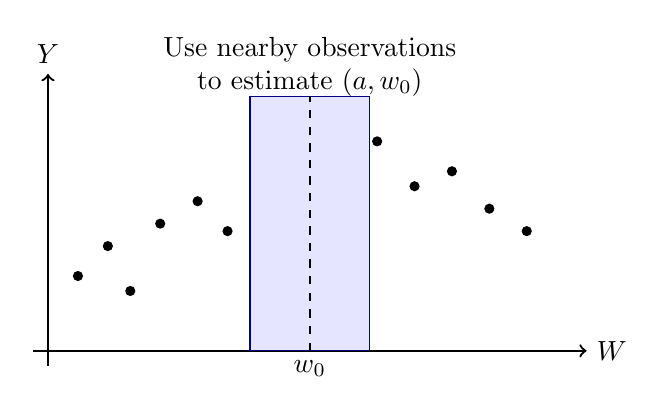
\begin{tikzpicture}[
  scale=.95,
  axis/.style={->, thick},
  pt/.style={circle, fill=black, inner sep=1.3pt},
  window/.style={fill=blue!10, draw=blue!50!black},
  arr/.style={-{Latex[length=2.5mm]}, thick}
]
\draw[axis] (-.2,0) -- (7.2,0) node[right] {$W$};
\draw[axis] (0,-.2) -- (0,3.7) node[above] {$Y$};
\foreach \x/\y in {.4/1.0,.8/1.4,1.1/.8,1.5/1.7,2.0/2.0,2.4/1.6,2.8/2.4,3.2/2.7,3.5/2.5,3.9/2.9,4.4/2.8,4.9/2.2,5.4/2.4,5.9/1.9,6.4/1.6}
  \node[pt] at (\x,\y) {};
\draw[window] (2.7,0) rectangle (4.3,3.4);
\draw[dashed, thick] (3.5,0) -- (3.5,3.4);
\node[below] at (3.5,0) {$w_0$};
\node[align=center] at (3.5,3.8) {Use nearby observations\\to estimate $\Qbar(a,w_0)$};
\end{tikzpicture}
\caption{Flexible regression borrows information across covariate values.}
\label{fig:ch5-borrowing}
\end{figure}

\subsection{Regression as Smoothing}

Regression is a formal way to borrow information. A regression estimator smooths the
observed outcomes across covariate values in order to estimate a conditional mean
function. The amount and shape of smoothing depend on the method.

A linear regression with
\[
\Qbar(a,w)=\beta_0+\beta_1a+\beta_2w
\]
borrows information very aggressively. The model assumes that a one-unit change in
$W$ has the same additive association with $Y$ everywhere. If this is true, the method
can be efficient. If it is false, the method may be biased.

A kernel regression borrows information locally. It estimates $\Qbar(a,w)$ using
observations whose covariates are close to $w$. A regression tree borrows information
within leaves of a fitted tree. A random forest averages many such trees. A generalized
additive model borrows information through smooth functions of predictors. Each
method embodies a different answer to the same question: which observations should
inform the prediction at a given covariate value, and how much should they count?

\subsection{Why Model Choice Matters for Causal Estimators}

In causal inference, nuisance regression quality matters because causal estimators are
functions of these regressions. For g-computation,
\[
\widehat{\ATE}_{\mathrm{gcomp}}
=
\frac{1}{n}\sum_{i=1}^n
\left\{\Qbar_n(1,W_i)-\Qbar_n(0,W_i)\right\}.
\]
If $\Qbar_n$ is biased in regions of the covariate space that are common in the target
population, the ATE estimate can be biased.

For IPTW,
\[
\widehat{\ATE}_{\IPTW}
=
\frac{1}{n}\sum_{i=1}^n
\left\{
\frac{\ind(A_i=1)}{g_{n,1}(W_i)}Y_i
-
\frac{\ind(A_i=0)}{g_{n,0}(W_i)}Y_i
\right\}.
\]
If $g_n$ is poorly estimated, the weights can be wrong, unstable, or both.

\begin{assumptionbox}
Flexible regression does not replace causal assumptions. Consistency,
conditional randomization, and positivity are still required to interpret the resulting
statistical estimates causally. Super Learning helps estimate observed-data nuisance
functions; it does not make unmeasured confounding disappear.
\end{assumptionbox}

\begin{estimationbox}
The practical objective in this chapter is to estimate nuisance functions well enough
for causal estimation. We therefore need a principled way to compare candidate
regression estimators before using them inside g-computation, IPTW, or later doubly
robust estimators.
\end{estimationbox}
